\chapter{Flowsheeting}

\begin{overview}
  Even though many representations of chemical processes are possible
  in theory, the flowsheet is the most popular in practice.  Process
  engineers use process flow diagrams and piping and instrumentation
  diagrams to document processes and flowsheeting software leverages
  their familiarity with the flowsheet format to represent the
  processes being simulated.  An overview is given here of
  flowsheeting terminology and common unit operations, along with
  common methods of solving dynamic and stationary flowsheeting
  problems.
\end{overview}

\section{Background}
%TODO: This is from the ESCAPE-19 article - incorporate
Flowsheeting has assumed a central position in modern process engineering practice.  
Diagrams describing the flow of material and energy through a plant are the main mode of communicating process design and several packages exist that solve the associated equations.
Steady state flowsheeting is accepted in industry to such an extent that it is unlikely that a chemical plant of any size is designed without the use of at least one such tool.~\citep{glasscock.hale1994process}

Market penetration of dynamic simulation is lagging behind that of steady state simulations, partly due to the computational requirements associated with such simulation and partly due to the considerable additional effort involved in developing dynamic simulations.
However, interest has increased in the development of dynamic plant simulations.  
In addition to dedicated process engineering tools like Aspen, ChemCAD, HYSYS/Unisim (Honeywell's Unisim software is based on HYSYS), ProSim and SimSci, several modelling languages have emerged in the last 15 years that aim to provide an environment for modelling dynamic processes.  
Ascend and gPROMS are two examples of this approach (see~chapter\ref{chap:software} for more discussion of simulation software). 
On another front, modelling systems have been developed for multi-discipline simulation.  
Modelica was specifically designed as a standard for such simulation, incorporating aspects from other languages~\citep{elmqvist.ab1997modelica,tiller.ph-d-2001introduction}.  
Modelica is a language, but is supported by graphical tools like Dymola, which allows a blend of graphical model-building and traditional programming.

The OpenModelica project provides an Open Source implementation of a Modelica compiler and environment, allowing researchers in the field of simulation to access and tinker with the underlying simulation code instead of only working on models.  
This allows flexibility beyond that afforded by commercial simulation packages which are primarily focused on providing a stable environment for simulation of new processes rather than new simulation approaches for existing processes.

The proprietary system gPROMS already has CAPE-OPEN support, and adding support for some CAPE-OPEN interfaces to OpenModelica may speed adoption of this open standard in the Process Engineering field.

Simulation of a distillation column has been done before in Modelica~\citep{duro.morilla2003modelling}.
However, the modelling strategy followed here is more modular, and abstracts the thermodynamics to the streams, allowing easy interfacing with an external thermodynamics package.

\section{Basic modelling equations}
Several equations are used in many different pieces of equipment
\subsection{Conservation of mass}
\subsection{Conservation of energy}
\subsection{Reaction kinetics}



\subsection{Equilibrium}
\subsection{Transport equations}
\subsubsection{Heat transfer}
\subsubsection{Mass transfer}

\section{Simulation}

\subsection{Modelling}
\citet[177]{giordano.fox.ea2009first} explains that numeric simulation is often required where analytic solution of modelling equations is not available.  

\subsubsection{Microscopic}

\subsubsection{Macroscopic}
Macroscopic modelling 

\subsubsection{Lumped models}


\section{Unit operations}
The concept of unit operations has been embedded in Chemical Engineers' psyche since Arthur D. Little coined the phrase in 1915~\citep{hougen1972seven}.  
Unit operations lend themselves to an object-oriented programming style, with their main functions encapsulated in a ``black box'', with narrow interfaces between them.
The following main unit operations are identified, following the sequence used in~\citet{msh}.

\subsection{Fluid flow operations}
These operations are further subdivided based on the nature of the
fluid flowing in them.  Uncompressible and compressible single phase
flow are the most commonly modelled types; multiphase flow is commonly
encountered in industry, but presents significant modelling
challenges.\citehere.

\subsubsection{Fluid movers}
This category encapsulates pumps, blowers, compressors and similar
equipment which bring about a change in momentum of a fluid by doing
work on it.  

\subsubsection{Valves}


\subsubsection{Pipes}


\subsection{Heat transfer}
\subsubsection{Heat exchangers}


\subsection{VLE}
Mass transfer operations 


\subsection{The phase rule}
%TODO: Find more fundamental reference
The phase rule can be stated as \citep[499]{mccabe.smith.ea1993unit}
\begin{equation}
  \label{eq:phaserule}
  F = C - P + 2
\end{equation}
Where $F$ is the degrees of freedom, $C$ is the number of components and $P$ the number of phases in equilibrium.  
Note that this relationship does not hold for reacting systems.

\subsubsection{Flashing}
A flash drum is a unit that separates a stream into a vapour and
liquid fraction based on the difference in composition of vapour and
liquid in phase equilibrium.  Figure~\ref{fig:flashdrum} shows a flash
drum with the relevant variables.

\begin{figure}[htbp]
  \centering
  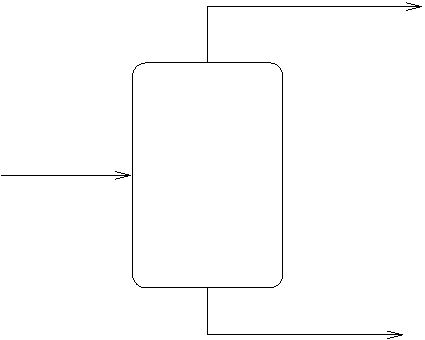
\includegraphics[width=0.4\textwidth]{flashdrum}
  \caption{Flash drum}
  \label{fig:flashdrum}
\end{figure}

The following assumptions are common when modelling flash drums:

\begin{itemize}
\item The phase equilibrium is achieved fully and quickly relative to
  the dynamics of the level of the flash drum.
\item The pressure in the flash drum changes only due to changes in
  the vapour balance.
\end{itemize}

Under these assumptions, the equations describing the dynamic
behaviour of a standard flash drum are given below (from \citet{eich-soellner.lory.ea1997stationary}):

\begin{align}
  \dxdy{M}{t}          & = F - V - L                                         \\
  \dxdy{M\vec{x}}{t}   & = Fx_j - Vy_j - Lx_j \text{ for } j = 1,\dots,n_c-1 \\
  \sum_{j=1}^{n_c} x_j & = 1                                                 \\
  \sum_{j=1}^{n_c} y_j & = 1                                                 \\
  y_j                  & = K_j(T, P, x, y)x_j \text{ for } j = 1,\dots,n_c-1 \\
  L                    & = \Phi(M)                                           \\
  \dxdy{Mh_L}{t}       & = Fh_F - Vh_V - Lh_L + Q                            \\
  h_p                  & = h_p(T_p, P_p, x) \text{ for } i \in {L, V}        \\
  P_V                  & = P_L = P                                           \\
  T_V=T_L=T
\end{align}

\subsection{Distillation}

The vapour-liquid equilibrium-based separation obtained in a flash unit can be
repeated an arbitrary number of times to obtain better separation as
long as the equilibrium allows for enrichment of the vapour.  A
distillation column is an integrated system allowing for repeated
equilibrium stages.  Liquid flows down the column under the influence
of gravity and vapour flows upward due to the difference in density
between the vapour and the liquid.  The vapour contacts with the
liquid on plates or on the surface of a packing material.  

A plated column can be described by similar equations as the flash
drum unit already discussed, with some coupling between the plates.
The amount of liquid on a column plate is called the holdup.

The following needs to be taken into account:



The flow of liquid down the column is a hydraulic prolem, involving
the flow over a weir.  The Francis weir formula describes this flow.


\subsection{Chemical reaction operations}
\citet[347]{cellier1991continuous} explains the modelling of chemical reactions in much detail, with reference to some of the following concepts:

\subsubsection{Stoicheometry}
Given a system of reactions such as:
\begin{equation}
  xA_iB_j -> yA_k + zB_lA_m,
\end{equation}
it is required that the reaction ``balances'', that is that the number
of atoms of A and B are unchanged by the reaction.  In the above case,
this implies that $xi=yk+zm$ and $xj=zl$.  It is usually desired to
find integer solutions for $x$, $y$ and $z$ given $i$ to $m$.  This is
known as balancing the reactions.  Once such solutions have been
found, they are known as the stoicheometric coefficients of the
reaction scheme.  It is useful to group the stoicheometric
coefficients into a stoicheometric matrix $\alpha$ such that the
magnitude of $\alpha_{i,j}$ is the coefficient of component $j$ in
equation $i$ ($x$ in the example above) and the sign of $\alpha_{i,j}$
is negative for reactants and positive for products.  Using this
notation, the following equations must hold at any time:
\begin{equation}
  \sum_{j=1}^{n_c} \alpha_{i,j}A_j = 0,~i=1,\dots,M
\end{equation}
Here, $A_j$ is the amount of component $j$ and $M$ is the  number
of reactions.

\subsubsection{Reaction rates}
Reaction rates are commonly modelled using the notation
$r_i=-\dxdy{C_i}{t}$, where $r_i$ is the reaction rate and $C_i$ is the
concentration of component $i$.  

Reaction rates are often given by a power law rate equation
\begin{equation}
  r_i = k_i \prod_{j=1}^{n_c}c_j^{\beta{i,j}} - k'_i\prod_{j=1}^{n_c}c_j^{\gamma{i,j}}
\end{equation}

The order 

\subsubsection{Rate constants}

\subsubsection{CSTR}

% TODO: look at http://gaia.lbl.gov/bie/modelica/msl/3.1/help/Modelica_Fluid_Examples_DrumBoiler_BaseClasses.html

\section{Dynamic flowsheeting}
\subsection{History}
The following time line shows major visible developments of
flowsheeting. \cite{husain1986chemical,mallja2000}
\begin{description}
\item[1955] Single unit steady state solutions 
\item[1958] Kelloggs - Flexible Flowsheet Program 
\item[1965] PRODYC dynamic simulator. 
\item[1970] IBM releases  first Personal Computer 
\item[1982] Speed-up dynamic simulator 
\item[1995] Aspen  Dynamic - includes GUI and full reporting of dynamic variables, including optimisation.
\end{description}

\section{Solving flowsheeting problems}
``Solving'' a flowsheet means solving for unknown variables given the knowns, either for a particular steady state value or over time given a dynamic model.  
This is also commonly called \emph{simulation} of the flow sheet.

\subsection{Specification}
\subsection{Static data requirements}
These properties are part of the setup of the problem
\begin{itemize}
\item Connections between units (unit input/outputs and mass or heat connections)
\item Physical properties of all pure substances
\item Macroscopic mixture properties - VLE, heat of solution, etc
\item Enough known values to satisfy a degrees of freedom analysis
\end{itemize}

Additional static data requirements for dynamic control
\begin{itemize}
\item Pure dead time as a separate characteristic.
\item Dead time of connections (effects of piping on control can be large).
\end{itemize}

Equation requirements
\begin{itemize}
\item Steady state energy and mass balances for each block.
These equations include links to other units that have to be resolved using tear streams to isolate blocks or by combining the whole problem into one matrix.
\item State equations using the constants defined in the static data.
\end{itemize}

Additional equation requirements
\begin{itemize}
\item Dynamic energy and mass balances for each block.
  These may be linear transfer functions or nonlinear differential equations.
\item State equations include dynamics, such as phase changes. 
\item Microscopic state equations modelling dynamic changes in properties.
\end{itemize}

\subsection{Steady state simulation}
Since the advent of programmable computers, they have been employed to solve routine design problems like mass and energy balances and rudimentary mechanical design issues.  
As the speed of these computers increased, programs were developed to include more complex problems. 
This led to the development of several flowsheeting programs.  
These programs solve the steady state equations of a number of unit operations connected to one another.  
This problem is also called steady state simulation \citep{westerberg.hutchison.ea1979process}

During the first years of flow sheeting, the main drive was towards a program that could solve the equations quickly.  
Once methods had been developed to do this, the focus moved toward speeding up the process involved in defining the problem.  
Interfaces progressed from simple parsers that forced the user to state the problem in a non-intuitive way using specific programming languages to the graphical user interfaces we know today.  
While the redesign of the interface was underway, an expansion of the existing technology was proposed by widening the problem from steady state to dynamic simulation.

\subsection{Dynamic simulation}
Computers were becoming more prevalent in the engineering community and several engineers concerned with process control were writing purpose-built dynamic simulations of unit processes to test control systems.  
Up to the mid 60s, analog computers were used to model dynamic systems \citep{husain1986chemical}, but as digital computers became more advanced, it seemed natural to expand the existing steady state flow-sheeting programs, to include dynamic behaviour. 
The problems involved in the expansion can be classified into three general classes: static data requirements, dynamic equation requirements and solution methodology.

\subsection{Solution methods}
Simulation of dynamic models usually begins with solution of the steady state problem by the normal methods employed in the steady state software.  
The solution of these equations supplies the program with the starting values needed to integrate the describing differential equations numerically.  
For a simply connected (non-cyclic) problem, numerical methods may be employed to integrate the equations in the order that the units are connected.  
When there is recycle of materials or heat integration between units, care must be taken to ensure that the interconnected quantity is consistently solved.  
In other words, units must be reconciled in some way to ensure that shared quantities are the same.  
Different solution methods solve this problem in different ways.

In the first approach, units are coupled at each solution step.  
This method has good accuracy but the extra time needed in each integration time step to reconcile units increases solution time dramatically.
Secondly, units may be separately solved and reconciled at the end of each integration time step.  
This method has very low accuracy for large time steps periods, but the increase in calculation speed also allows lower integration time steps~\citep{husain1986chemical}.  
Both of these methods follow a modular approach: each module is solved independently and then reconciled with the other units.

The third method involves setting up a total set of equations based on the module equations and integrating the total system.  
This method is currently favoured by the simulation community, as there are several applications of parallel processing and large vector computers and networks for the solution of these systems, which are usually large but sparse (Malja et al, 2000).

The extension to the solution methodology is so great that it may not seem an extension, but rather a new problem altogether.  
Many of the traditional methods used to solve the steady state problem are no longer relevant as computer speed improves.  
Tear stream identification and similar techniques to decouple units have been largely replaced by the method mentioned above.

\section{Modelling}
\begin{figure}[htp]
  \centering
  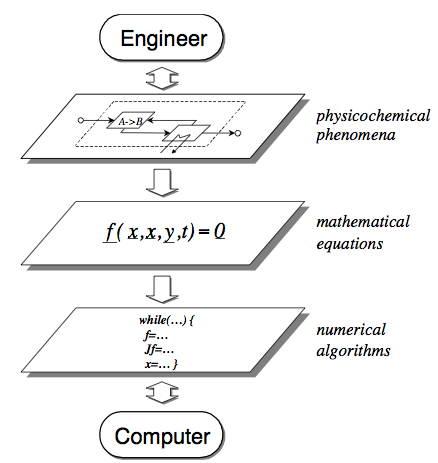
\includegraphics[width=0.5\textwidth]{modelling_flow}
  \caption[Modelling process]{Modelling process as explained by \citet{biezczad}}
  \label{fig:modellingprocess}
\end{figure}

% Local Variables:
% TeX-master: "thesis"
% End:

